\documentclass{beamer}
\usepackage[T1]{fontenc}

\usepackage[utf8]{inputenc}
\usepackage[english,italian,icelandic]{babel}
\usepackage{CJKutf8}
%\usepackage[italian]{babel}

\usetheme{Unicam}

\usepackage{listings}

\lstset{ %
    basicstyle=\tiny\ttfamily,
    frame=single,
    language=Python,
    commentstyle=\itshape\color{green!40!black}
}

\usepackage{float}
\usepackage{wrapfig}
\usepackage{graphicx}
\graphicspath{{img/}}
\usepackage{caption}
\usepackage{multicol}
\captionsetup{
  font=scriptsize,
  labelfont=scriptsize
}

\author{fales}%
\title{Real-time Online Multiplayer with Godot Engine}
\university{}%
\school{}%
\course{}%
\academicyear{February, 2017}%
\date{\today}
\definecolor{schoolbgcolor}{HTML}{D71921}
\definecolor{schoolfgcolor}{HTML}{FFFFFF}

\newcommand{\tlink}[3] {
 \href{#1}{\textbf{#3}}

 \href{#1}{#2}
}

\newcommand{\slink}[2] {
 \href{#1}{#1}

 \href{#1}{\footnotesize{#2}}
}

\begin{document}

\begin{nohead}
  % Frontespizio
  \begin{nofoot}
  \frame{\titlepage}
  \end{nofoot}

  % Table of content
  \begin{frame}{}
    \begin{multicols}{2}
      \setcounter{tocdepth}{2}
      \tableofcontents
    \end{multicols}
  \end{frame}
\end{nohead}

\section{Introduction}
\subsection{Goals}
\frame{\frametitle{Goals}


\footnotesize{
    \begin{itemize}
        \item Having multiple persons \textbf{playing the same game together}, on different machines, \textbf{through a network}.
        \item \textbf{No apparent input delay}: Players must feel like they are playing the game on their computer
        \item \textbf{No apparent lag or video delay}: Players should experience a good simulation
        \item \textbf{No cheaters}: Players should not be allowed to do or see anything besides what allowed by the game
    \end{itemize}
}

}
\subsection{Problems}
\begin{frame}{The Internet is not a pipe}


\begin{columns}[T]
  \begin{column}{.3\textwidth}
    \begin{block}{}


\begin{figure}[htbp!]
  \begin{center}
    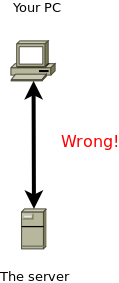
\includegraphics[width=.6\textwidth]{pipe}
    \caption*{\tiny{This is wrong}}
   \end{center}
\end{figure}

    \end{block}
  \end{column}
  \begin{column}{.7\textwidth}
    \begin{block}{}
    
\begin{figure}[htbp!]
  \begin{center}
    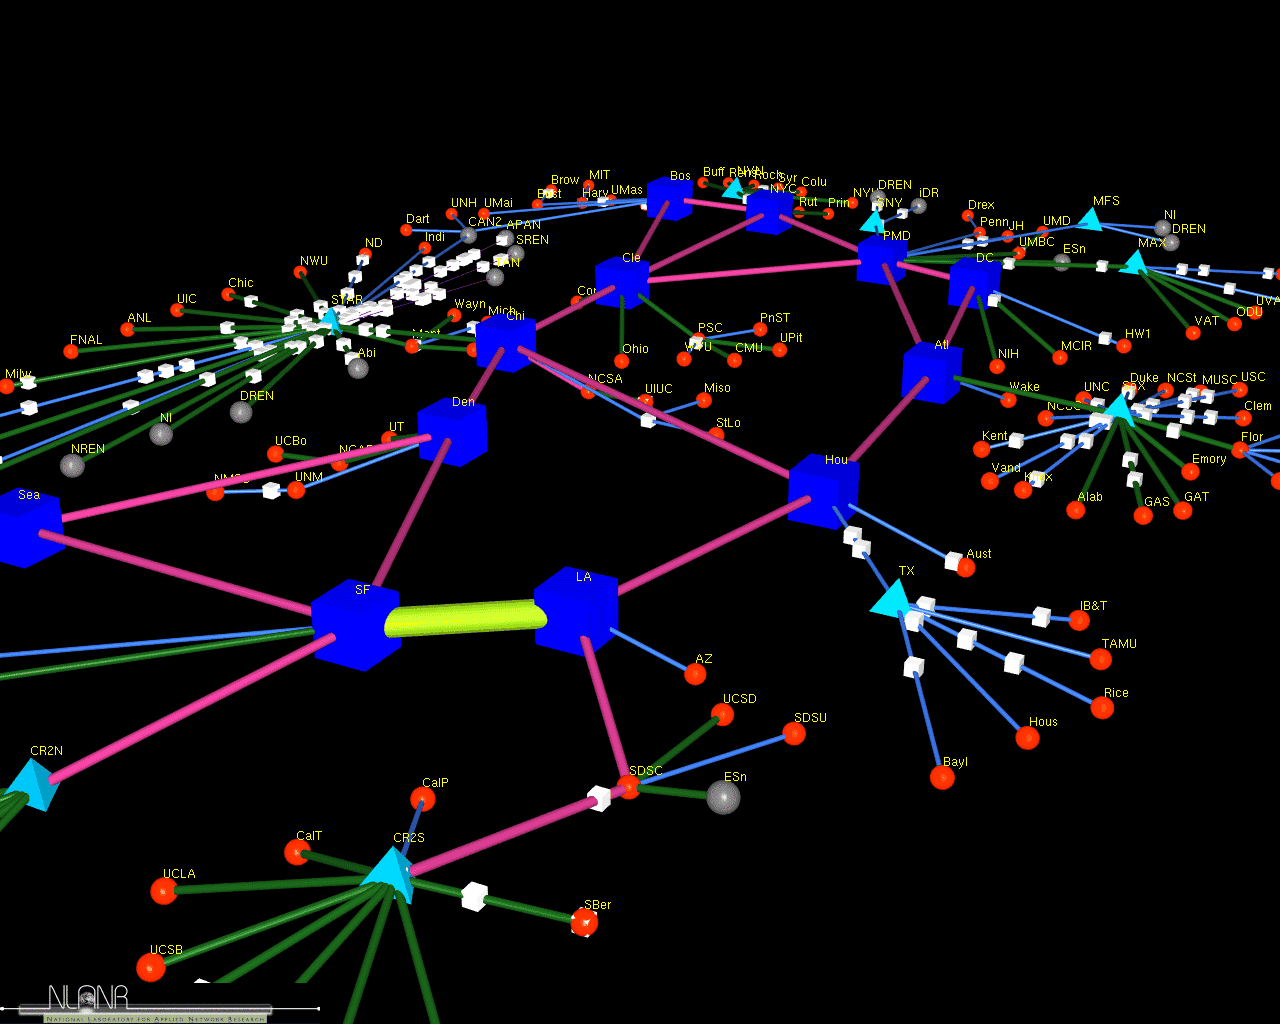
\includegraphics[width=.8\textwidth]{internet}
    \caption*{\tiny{This is more like it}}
   \end{center}
\end{figure}

    \end{block}
  \end{column}
\end{columns}

\end{frame}
\frame{\frametitle{Problems}

\begin{itemize}
    \item Networks are unreliable (packets can take different route and arrive out of order or get lost)
    \item Networks have limited data rate and can be slow or become clogged
    \item Networks add delay (even the light takes time, imagine a decades old copper twisted pair)
\end{itemize}

}
\subsection{Guidelines}
\frame{\frametitle{Guidelines}

There is no one fit all solution.

It really depends on you game. (genre, mechanics, interactions).

There are a few general guidelines

\begin{itemize}
    \item Everything should happen on the server, clients are mere dummy displays.
    \item Clients should only send their inputs or commands (server must discard disallowed commands)
    \item Send as little data as possible as often as possible to keep latency at a minimum for RT games.
\end{itemize}

}
\subsection{Common techniques}
\frame{\frametitle{Common techniques}

\begin{columns}[T]
  \begin{column}{.6\textwidth}
    \begin{block}{}

\begin{itemize}
    \item UDP Networking
    \item State synchronization
    \item Interpolation
    \item Compression/Size optimizations
    \item Lag compensation
\end{itemize}

    \end{block}
  \end{column}
  \begin{column}{.4\textwidth}
    \begin{block}{}

\vspace{-1.5cm}

\begin{figure}[htbp!]
  \begin{center}
    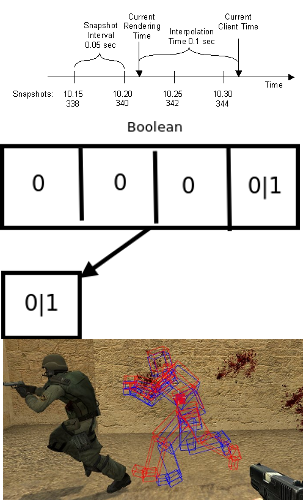
\includegraphics[width=1\textwidth]{tech}
    \caption*{\tiny{Common techniques}}
   \end{center}
\end{figure}

    \end{block}
  \end{column}
\end{columns}

}
\subsection{TCP vs UDP}
\begin{frame}[t]{TCP vs UDP}

\vspace{-1cm}

\begin{columns}[t]
  \begin{column}{.5\textwidth}
    \begin{block}{}
    \large{TCP}

    \begin{itemize}
        \item Connection based
        \item Reliable delivery
        \item Ordered delivery
        \item High latency
    \end{itemize}
    \end{block}
\end{column}
  \begin{column}{.5\textwidth}
    \begin{block}{}
    \large{UDP}
    \begin{itemize}
        \item Connectionless
        \item Unreliable delivery
        \item Unordered delivery
        \item Low latency
    \end{itemize}
    \end{block}
  \end{column}
\end{columns}

\end{frame}

\section{Godot Low Level Networking}
\subsection{Server}
\begin{frame}[fragile]{Godot low level UDP}

Echo Server

\begin{lstlisting}
var _clients = []
var _udp = PacketPeerUDP.new()

func _ready():
    _udp.listen(4321)
    set_process(true)

func _process(delta):
    var msgs = []

    while _udp.get_available_packet_count() > 0:
        var pkt = _udp.get_var() # or get_packet()
        var ip = _udp.get_packet_ip()
        var port = _udp.get_packet_port()
        if _clients.find(ip + ":" + str(port)) == -1:
            # New client
            _clients.append(ip + ":" + str(port))
        # Prepare message to be broadcasted
        msgs.append(ip + ":" + str(port) + "-" + str(pkt))
    # Broadcast messages
    for c in _clients:
        var splitted = c.split(":")
        _udp.set_send_address(splitted[0], int(splitted[1]))
        for msg in msgs:
            _udp.put_var(msg)
\end{lstlisting}

\end{frame}
\subsection{Client}
\begin{frame}[fragile]{Godot low level UDP}

Client

\begin{lstlisting}
var _udp = PacketPeerUDP.new()

func _ready():
	_udp.set_send_address("localhost",4321)
	set_process(true)

func _process(delta):
	var msgs = []

	while _udp.get_available_packet_count() > 0:
		var pkt = _udp.get_var() # or get_packet()
		msgs.append("Server says: " + str(pkt))
	# Show messages
	for msg in msgs:
		print(msg)

func send_data(data):
	_udp.put_var(data) # or put_packet
\end{lstlisting}

\end{frame}
\subsection{Problems}
\frame{\frametitle{Problems with UDP}

\begin{itemize}
    \item Detect client disconnection (ping/timeout)
    \item Detect out of order packets (time sync)
    \item Detect/resend packet lost if we want it to be reliable (sequence/acks)
\end{itemize}

}
\subsection{Solutions}
\frame{\frametitle{Some solutions}

\begin{itemize}
\item Have the client sends some \textbf{ping packet}, if a ping is \textbf{not received} by the server for \textbf{more than X seconds}, the client is considered \textbf{disconnected}
\item Send and additional \textbf{time} value with packets you want to be ordered.
    \textbf{Keep} the \textbf{last received} time, if you receive a \textbf{lower time}, \textbf{drop it}. (see wrap)
\item Have the two parties add sequence numbers to pacekets and \textbf{send acknowledgment} of received data. \textbf{Keep a queue} of last sent/received packets. Stop sending until you receive an ack for the lowest missing packet if the new packet has a sequence number higher than the lowsest plus the ack window size. Reorder received packets... \textbf{mess}!
\end{itemize}

\footnotesize{\textbf{Note:} have a look at \emph{var2bytes} and \emph{bytes2var}}

}

\addcontentsline{toc}{subsection}{\vspace{2cm}}

\section{Godot High Level Networking}
\begin{frame}{Godot High Level Networking}

\begin{itemize}
    \item Based on ENet library (might change in the future or on specific platform)
    \item Allow both reliable and unreliable communication over UDP
    \item Based on RPC calls
\end{itemize}

\vspace{1cm}

\tiny{
\textbf{See} \href{http://docs.godotengine.org/en/latest/tutorials/high\_level\_multiplayer.html}{http://docs.godotengine.org/en/latest/tutorials/high\_level\_multiplayer.html}
}

\end{frame}
\begin{frame}{Godot High Level Networking II}

Node network modes:

\begin{itemize}
    \item Master: This node is considered master (this instance owns it)
    \item Slave: This node is considered slave (someone else owns it)
\end{itemize}

RPC/RSET modes:

\begin{itemize}
    \item sync: called both locally and over network
    \item remote: called only remotely (no matter the owner)
    \item slave: the function will be called only on slave nodes
    \item master: the function will be called only on the master node
\end{itemize}

\end{frame}
\subsection{Server}
\begin{frame}[fragile]{Server}

\begin{lstlisting}
func create_server():
	set_network_mode(NETWORK_MODE_MASTER)
	var host = NetworkedMultiplayerENet.new()
	host.create_server(4321, 4)
	get_tree().set_network_peer(host)

var time = 0
func update_remote_state(tick): # Tick is ideally 20/30 FPS (ie. 0.05/0.03)
	var state = []
	# Parse the game state
	# ... eg.
	state.append(get_pos())
	state.append(get_linear_velocity())
	# Send RPC, called on the node with the SAME PATH in the client
	time += 1
	rpc_unreliable("update_state", time, tick, state)

slave func update_state(time, tick, state):
	# ... (see next slide)

\end{lstlisting}
 
\end{frame}
\subsection{Client}
\begin{frame}[fragile]{Client}
    
\begin{lstlisting}
func create_client():
	set_network_mode(NETWORK_MODE_SLAVE)
	var client = NetworkedMultiplayerENet.new()
	client.create_client("127.0.0.1", 4321)
	get_tree().set_network_peer(client)

var last_time = 0
slave func update_state(time, tick, state):
	# Handle wrap-around, see rfc1185 as reference
	if last_time >= time: # Out of order packet... drop
		return
	last_time = time
	# Handle state update here eg. tween this object
	get_node("Tween").stop_all()
	get_node("Tween").interpolate_method(self, "set_pos", 
                                        get_pos(), state[0]], tick,
                                        Tween.TRANS_LINEAR, Tween.EASE_IN)
	get_node("Tween").interpolate_method(self, "set_linear_velocity", 
                                        get_linear_velocity(), state[1], tick, 
                                        Tween.TRANS_LINEAR, Tween.EASE_IN)
	get_node("Tween").start()
\end{lstlisting}

\footnotesize{\textbf{Note}: the node that makes the RPC MUST have the same node path for in both server and client for this to work}
    
\end{frame}
\subsection{Optimizations}
\begin{frame}{Optimizations?}

\begin{itemize}
    \item Try to bundle homogeneous data in the same state update (but make sure the maximum packet size will be less than 400-450 bytes, or it might get dropped).
    \item Optimize your state update! (see note, eg. boolean can be 1 byte instead of 4)
    \item Use prediction! \\
    \footnotesize{Instead of interpolating \texttt{recv\_pos} and \texttt{recv\_vel}, interpolate to \texttt{recv\_pos + recv\_vel * tick} , and keep predicting till next frame}
\end{itemize}


\href{http://docs.godotengine.org/en/stable/reference/binary_serialization_api.html}{\tiny{\textbf{Note}: http://docs.godotengine.org/en/stable/reference/binary\_serialization\_api.html}}

\end{frame}

\section{Benet module}
\begin{frame}{Benet module}

\begin{itemize}
    \item Developed to use ENet at full power
    \item Does not use RPC (unless you want to)
    \item Allow for \texttt{broadcast} \texttt{send} (to specific client)
    \item Uses signals to notify of recv packets, clients connect/disconnect
    \item Allow for unreliable but ordered channels (you don't have to manage time)
    \item Allows multiple channels
\end{itemize}

\footnotesize{\textbf{Note}: will likely not be included in Godot, I'm looking to port it to the C API by \textbf{karroffel} and \textbf{bojidar-bg} when it's ready}

\end{frame}

\section{End}
\frame{\frametitle{}

\begin{center}

\textbf{Thanks for your time!}

\vspace{1cm}

\textbf{Questions?}

\vspace{1cm}

\textbf{Useful link:}

\vspace{0.1cm}

\slink{http://gafferongames.com/networking-for-game-programmers/}{\vspace{.1cm}Gaffer on Games - Game Networking}

\slink{https://developer.valvesoftware.com/wiki/Lag\_compensation}{Valve Wiki - Lag compensation}

\end{center}

}

\end{document}
